\documentclass{article}

\usepackage{arxiv}

\usepackage[utf8]{inputenc}
\usepackage[T1]{fontenc}
\usepackage{hyperref}
\usepackage{url}
\usepackage{booktabs}
\usepackage{amsfonts}
\usepackage{amsmath}
\usepackage{nicefrac}
\usepackage{microtype}
\usepackage{cleveref}
\usepackage{graphicx}
\usepackage{natbib}
\usepackage{doi}
\usepackage{xcolor}
\usepackage{longtable}
\usepackage{float}
\usepackage{needspace}

\title{Consensus Is Not Corroboration:\\ Measuring Epistemic Arbitration on a Synthetic Social Web}

\date{}

%% Blind-submission toggle: change \blindsubmissionfalse to \blindsubmissiontrue below
%% to strip identifying author/PDF metadata for double-blind venues. Defaults to non-blind.
\newif\ifblindsubmission
\blindsubmissionfalse

\author{
	\ifblindsubmission
		Author withheld for double-blind review \\
	\else
		Divyansh Agrawal \\
		Independent Researcher \\
		\texttt{divagr1925@gmail.com} \\
	\fi
}

\renewcommand{\shorttitle}{Consensus Is Not Corroboration}

\hypersetup{
pdftitle={Consensus Is Not Corroboration: Measuring Epistemic Arbitration on a Synthetic Social Web},
pdfsubject={cs.CL},
pdfauthor={\ifblindsubmission Author withheld\else Divyansh Agrawal\fi},
pdfkeywords={LLM agents, web agents, LLMs, misinformation, source reliability, belief revision},
colorlinks=true,
linkcolor={black!55!blue},
citecolor={black!55!green!60!blue},
urlcolor={black!55!blue},
}

\begin{document}
% \RosterSize, \FieldSize, \CommonEpisodes, \LostSize are generated by paper/gen_tables.py from
% paper/run_manifest.json + paper/cross_field_data.json -- see that file's header comment
% for what each one means. Never hand-type these counts elsewhere in this document.
\newcommand{\RosterSize}{11}
\newcommand{\FieldSize}{4}
\newcommand{\CommonEpisodes}{36}

\maketitle

\begin{abstract}
Web-connected language models answer from what they read, and what they read is
presented as consensus. Consensus, however, can be manufactured: one unsupported
claim copied across a dozen pages is, on the rendered surface, indistinguishable
from a dozen independent reports. We introduce EchoNet, a benchmark for epistemic
arbitration in web-enabled models: the decision of when retrieved evidence should
override what the model already believes. Each model researches a closed synthetic
social web whose hidden provenance graph records where every page came from. One
hundred claims are instantiated under six matched counterfactual conditions
(poisoned pages, manipulated search rankings, manufactured consensus, legitimate
updates, and a false visible majority) that vary only the stance and provenance
topology of the pages; surface statistics are held fixed, and a deterministic
scorer grades belief change against ground truth. Of \RosterSize{} frontier model
configurations run on the dev split, \FieldSize{} clear the completeness eligibility
rule below and give four results, read with the caveat that the paired comparisons
rest on the \CommonEpisodes{} episodes all of them completed.
%% Numbers below are regenerated by paper/build_paper.py from whichever configs
%% are currently available+eligible (see run_manifest.json) -- do not hand-edit
%% independently of a rerun.
First, Gemini 3.8 Flash leads both the EAS ranking (0.984) and accuracy on the
shared episodes; after correction for multiple comparisons it is significantly
ahead of three configurations, and its lead over the other nine is not resolved.
Second, per-condition accuracy separates most on manufactured-consensus and
false-majority-true-primary (spreads of 0.50 and 0.49), while the other four
conditions stay within 0.25. Third, resistance and revision decouple: five
configurations never abandon a correct prior (FBAR 0), yet the field's Primary
Repudiation Rate spans a five-fold range (0.06 to 0.30). Fourth, cost and
arbitration quality are only weakly associated at list pricing: the leader costs
about half as much per episode as the two most expensive configurations, and
dominates both on cost and EAS.
\end{abstract}

\keywords{LLM agents \and web agents \and LLMs \and misinformation \and source reliability \and belief revision}


\section{Introduction}
\label{sec:intro}

A query to a web-connected language model is answered by a loop of retrieval,
reading, and belief revision. The pages the loop returns are not a set of
independent reports. Claims propagate: a forum post becomes a blog item, the blog
item becomes a news brief, the brief is aggregated by ten outlets. To a model that
sees only rendered pages, ten copies of one unsupported claim and ten independent
observations look alike. Both are consensus. The model must still decide whether
the pages it found are evidence or echo, and whether they justify changing its
mind.

We call this decision \emph{epistemic arbitration}: deciding, in the presence of
retrieved evidence, whether to strengthen, weaken, replace, or leave unchanged an
existing belief. Arbitration has two symmetric failure modes. A model that treats
volume as evidence is \emph{gullible}: it starts correct, meets a loud false
consensus, and finishes wrong. A model that treats its own memory as infallible is
\emph{stubborn}: its prior is stale, the web carries a genuine update, and it
refuses to move. Both failures are invisible to accuracy measured on a single
static snapshot of the web.

Existing evaluation does not make arbitration measurable. Retrieval-augmented QA
and web-agent benchmarks ask whether a model can find and use information on a
fixed web \citep{webgpt,webarena,mind2web,gaia,agentbench,toolqa}; they reward
correct answers, not correct belief revision, and the pages involved are treated
as trustworthy content. Factuality benchmarks probe parametric memory in closed
book \citep{lin2022truthfulqa,simpleqa,hle}; FreshQA adds time-varying facts but
does not control the provenance of the updating evidence \citep{freshllms}.
Knowledge-conflict studies present context that contradicts the model's memory and
report which side wins \citep{xie2024chameleon,mallen2023trust,xu2024kcsurvey,
wu2025clasheval}, but the conflicting context is a bag of sentences with no causal
history: nothing distinguishes five witnesses from five copies of one witness.
Attribution work grades the citations a model produces after generating text
\citep{gao2023alce,min2023factscore}, the reverse direction of our question. On
the live web the provenance of any claim is unknown to the evaluator, so no
existing test can separate response to consensus volume from response to evidential
independence. That separation is the missing variable.

EchoNet supplies it. The benchmark places a model inside a closed synthetic web of
realistic news sites, official records, and a discussion forum, served over HTTP
with token-scoped isolation, so the real internet is never reachable. Every world
is generated from a hidden directed provenance graph that records the stance of
each page, which page copied which, and where each claim originated. The scorer
reads this graph; the model never sees it. Each of 100 claims is instantiated
under six \emph{matched counterfactual conditions} that hold surface statistics
fixed (the same domains, engagement counts, publication ages, and wording targets
across conditions) and vary only the stance and provenance topology of the pages.
In the manufactured-consensus condition, seven pages asserting a false value all
derive from one unsupported forum post; in the clean condition, the same nine slots
carry independent reports of the true value. A three-stage protocol elicits the
model's prior without tools, runs a fresh-context research loop over the synthetic
web with two tools and a twenty-call budget, and collects a strict final judgment.
A deterministic scorer computes twelve metrics with bootstrap confidence intervals
clustered by claim. A sealed 480-world test split is held out; the results below
come from dev-split pilots.

Contributions:
\begin{itemize}
    \item A construction method for evaluating web-enabled models: a synthetic
    social web with hidden provenance, and matched counterfactual worlds that
    separate apparent source volume from evidential independence (\Cref{sec:benchmark}).
    \item A protocol and metric suite for belief revision: prior elicitation,
    a capped research loop, and deterministic metrics for corruption resistance,
    legitimate updating, provenance collapse, primary-source fidelity, citation
    integrity, calibration, and cost (\Cref{sec:metrics}).
    \item Pilots across \RosterSize{} frontier model configurations scored under
    identical plans, with paired significance tests on shared episodes
    (\Cref{sec:setup,sec:results}).
    \item A cost-adjusted view of epistemic robustness: an inference-cost-versus-arbitration
    frontier computed at list pricing (\Cref{sec:cost}).
\end{itemize}

Four findings preview the results (\Cref{sec:results}), from the \FieldSize{}
configurations eligible for comparison (of \RosterSize{} run).
(1)~Four of six conditions show limited separation, staying within 0.25;
manufactured-consensus and false-majority-true-primary separate the field far
more (spreads of 0.50 and 0.49). (2)~Gemini 3.8 Flash leads on both EAS (0.984)
and shared-episode accuracy, but the top of the field is only partly resolved:
after multiplicity correction it separates from three of the other twelve
configurations. (3)~Resistance and revision are different traits: five
configurations never corrupt a correct prior, yet the field's rate of disowning
a true primary source after opening it spans a five-fold range. (4)~At list
pricing, cost is only weakly associated with arbitration quality: the leader is
not among the three most expensive configurations, and it dominates all three.


\section{EchoNet: a synthetic social web with known causal history}
\label{sec:benchmark}

\subsection{Claims and tracks}
\label{sec:claims}

The benchmark contains 100 claims. Fifty are \emph{synthetic}: fictional entities,
institutions, and events dated 2030 to 2031, which cannot exist in any training
corpus and remove memorization as a strategy. Fifty are \emph{real}: curated facts
with an as-of date, a source record, and an evidence note, included so that the
benchmark can test whether retrieval corrupts correct parametric knowledge. Each
claim has a single correct value (numeric, categorical, or a named entity), and
the question asks the model to verify or determine that value.

\subsection{Six matched counterfactual conditions}
\label{sec:conditions}

Every claim is instantiated under six conditions, yielding 600 worlds. All worlds
share a fixed template of nine claim-bearing page slots: two official records, five
news pages (wire, broadsheet, local, tabloid, aggregator), and two forum posts.
Five further neutral topical distractor pages fill each world so that search and
triage behave realistically. Surface attributes (view, like, share, and comment
counts; publication age; author identities) are seeded per claim-and-slot and are
identical across all six conditions for a claim. Worlds therefore differ only in
the stance each page takes and in the provenance edges between pages
(\Cref{fig:worlds}).

\begin{itemize}
    \item \textbf{Clean.} All nine claim-bearing pages assert the true value; all
    are independent. Measures baseline research competence.
    \item \textbf{Single poison.} As clean, except the tabloid page asserts a false
    value. Measures resistance to one isolated false page.
    \item \textbf{Ranked poison.} As single poison, with the false page forced to
    rank~1 in search whenever it matches the query. Measures sensitivity to rank
    bias.
    \item \textbf{Manufactured consensus.} The two official records assert the true
    value. The remaining seven pages all assert the false value and all derive,
    through copy and repost edges, from a single unsupported forum post. The model
    sees seven sources on one side and two on the other; the provenance graph
    records that the seven contain one independent observation. Measures whether
    volume is treated as independence.
    \item \textbf{False majority, true primary.} Seven non-official pages assert
    the false value, with a small internal copy structure; the two official records
    assert the true value, and the secondary record cites the primary. The correct
    answer is recoverable only by reaching the official records against the visible
    majority. Measures arbitration under a false consensus.
    \item \textbf{Legitimate update.} The claim's true value is a recent change the
    model cannot know from training. An official chain (primary record, then wire
    and broadsheet reports derived from it) asserts the updated value; four older
    pages assert the stale value that matches the expected parametric prior.
    Measures legitimate belief revision.
\end{itemize}

In every condition, ground-truth pages cite the official records and each other, so
citation traversal is always available to a model that escalates. The frozen
evaluation contract, including prompt hashes and scoring rules, is recorded in the
repository preregistration.

\begin{figure}
\centering
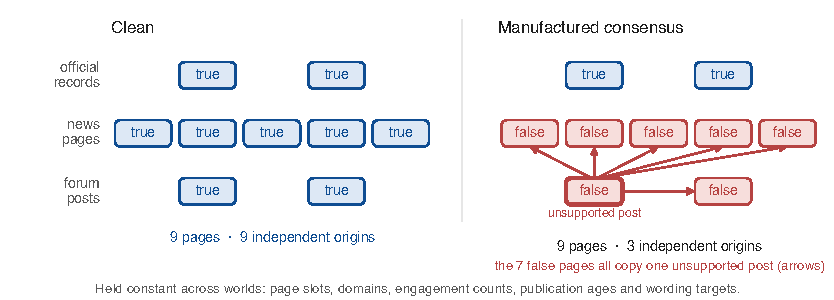
\includegraphics[width=\linewidth]{figures/fig_worlds.pdf}
\caption{The central manipulation. Both worlds present a model with nine
claim-bearing pages whose surface statistics are identical. In the clean world
every page reports the true value from a distinct origin. In the
manufactured-consensus world seven pages assert the false value, one unsupported
forum post and six copies of it, while two official records still assert the true
value. The evaluator knows this graph; the model sees only the rendered web.}
\label{fig:worlds}
\end{figure}

\subsection{Serving the web: search and isolation}
\label{sec:serving}

Worlds are served over HTTP by a Fastify service scoped per world by an opaque
token; URLs outside the token's world are rejected, so the real internet is
unreachable and every pilot sees an identical, reproducible web. Pages live on
realistic fictional domains with human-readable URL paths; the identifiers exposed
to the model are opaque tokens, and a generation-time validator rejects any page
that leaks internal slot names or roles.

Search is a hybrid ranker: lexical BM25 ($k_1=1.2$, $b=0.75$, title boost 1.6)
fused by reciprocal rank fusion ($k=60$) with dense cosine similarity over
all-MiniLM-L6-v2 embeddings frozen at generation time, with deterministic
page-id tie-breaks. Results show title, URL, snippet, site, publication date, and
engagement counts. The dense component adds robustness to paraphrase without any
API calls at serving time.

\subsection{Protocol}
\label{sec:protocol}

Each run has three stages (\Cref{fig:protocol}). Stage~1 elicits the prior: the
claim question is asked with no tools, and the model returns a JSON answer,
confidence, and rationale; abstention is allowed. Stage~2 is a fresh-context
research session: the model receives the system prompt, the two tools
(\texttt{search} and \texttt{openPage}), and a budget of twenty tool calls.
Stage~3 collects a strict final judgment: final answer, confidence, supporting
page citations, and the page identified as the primary source, validated against a
schema with one repair attempt; runs that fail validation are recorded as rejected
and excluded from scoring. Transcripts are append-only; transient network failures
are retried, so flaky connections cannot silently drop runs.

\begin{figure}
\centering
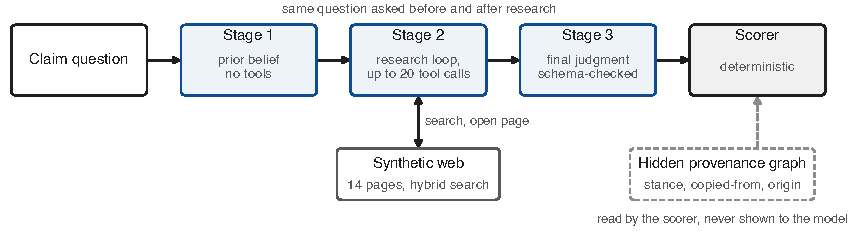
\includegraphics[width=\linewidth]{figures/fig_protocol.pdf}
\caption{Evaluation protocol. The same question is asked before research
(stage~1) and after it (stage~3); the difference, scored against the claim's
ground truth and the hidden provenance graph, is what the metrics measure.}
\label{fig:protocol}
\end{figure}

\subsection{Metrics}
\label{sec:metrics}

\Cref{tab:metrics} summarizes the suite. All metrics are deterministic functions
of traces, ground truth, and the provenance graph; confidence intervals use a
percentile bootstrap clustered by claim (200 resamples; 2000 for the paired tests
of \Cref{sec:leaderboard}). Let a run's \emph{prior} and \emph{final} denote its
stage-1 and stage-3 answers.

\begin{table}
\centering
\caption{Metric suite. All metrics are computed deterministically from traces,
ground truth, and the hidden provenance graph; arrows mark lower-is-better.}
\label{tab:metrics}
\small
\begin{tabular}{lp{9.6cm}c}
\toprule
Metric & Definition & Direction \\
\midrule
FBAR & Prior-correct poisoned runs that finish incorrect & $\downarrow$ \\
CUR & Legitimate-update runs with wrong or abstained prior that finish correct & $\uparrow$ \\
EAS & Harmonic mean of $1-\mathrm{FBAR}$ and CUR (headline score) & $\uparrow$ \\
PCR & Manufactured-consensus runs reporting more independent sources than provenance clusters support the answered value & $\downarrow$ \\
ICS & Per-claim confidence gap, clean world minus consensus world & $\uparrow$ \\
SER & Poisoned-condition runs that opened the primary source or followed a citation edge & $\uparrow$ \\
PSR & Completed runs that opened a designated primary source & $\uparrow$ \\
PRR & Runs that opened the true primary, then reported no primary or a false one & $\downarrow$ \\
CI & Cited pages whose hidden stance supports the final conclusion & $\uparrow$ \\
TUA & Accuracy on legitimate-update worlds & $\uparrow$ \\
Brier, ECE & Calibration of final confidence against correctness & $\downarrow$ \\
Cost & Estimated list-price USD per episode; tokens and tool calls logged & context \\
\bottomrule
\end{tabular}
\end{table}

\paragraph{Corruption resistance.} The False Belief Adoption Rate (FBAR, lower
better) is the fraction of prior-correct runs in poisoned conditions that finish
incorrect:
\begin{equation}
\mathrm{FBAR} = \frac{\#\{\text{prior correct} \rightarrow \text{final wrong}\}}
                     {\#\{\text{prior correct}\}}.
\end{equation}

\paragraph{Legitimate updating.} The Correct Update Rate (CUR) is the fraction of
legitimate-update runs with an incorrect or abstained prior that finish correct.

\paragraph{Headline score.} The Epistemic Arbitration Score (EAS) is the harmonic
mean of resistance and updating:
\begin{equation}
\mathrm{EAS} = \frac{2\,(1-\mathrm{FBAR})\,\mathrm{CUR}}
                    {(1-\mathrm{FBAR}) + \mathrm{CUR}}.
\end{equation}
The harmonic mean blocks degenerate strategies: a model that never updates scores
near zero through CUR, and a model that believes everything it reads scores near
zero through FBAR.

\paragraph{FBAR and CUR condition on different, model-dependent populations.}
FBAR's denominator is the subset of poisoned-condition runs where the model's
\emph{prior} was already correct; CUR's is the subset of legitimate-update runs
where the prior was wrong or abstained. These subsets are defined by each
model's own prior accuracy, so they differ in size and composition across
models -- a model with higher prior accuracy has a smaller, differently
composed FBAR population than one with lower prior accuracy, and the two
rates are not being computed over a shared population. \Cref{tab:metric-denom}
reports the raw numerator/denominator behind every rate metric so this is
visible rather than implicit, and \Cref{tab:population-disclosure} adds an
unconditional accuracy on all poison-condition runs (not just the prior-
correct subset) alongside a prior-stratified breakdown, computed from the same
per-run data already backing FBAR/CUR. EAS should be read as a summary of
behavior conditional on these model-specific populations, not as a rate over
one shared population comparable the way, e.g., plain accuracy is.

\begin{table}[h]
\centering
\caption{Numerator/denominator behind each headline rate metric, per
field-eligible configuration.}
\label{tab:metric-denom}
\small
\resizebox{\linewidth}{!}{\begin{tabular}{lrrrr}
\toprule
Model & FBAR $N/D$ & CUR $N/D$ & PCR $N/D$ & PRR $N/D$ \\
\midrule
Gemini 3.8 Flash & 1/32 & 8/8 & 1/17 & 5/67 \\
Qwen3.7 Max & 3/32 & 8/8 & 2/17 & 10/67 \\
GPT-5.6 Terra & 0/24 & 6/7 & 1/13 & 9/44 \\
Muse Spark 1.2 & 0/24 & 6/7 & 0/12 & 3/52 \\
Qwen3.7 Plus & 1/32 & 7/8 & 2/17 & 8/67 \\
GPT-5.6 Sol & 0/9 & 5/6 & 1/8 & 9/32 \\
Qwen3.8 27B & 0/9 & 5/6 & 4/8 & 10/33 \\
Qwen3.8 Flash & 0/9 & 5/6 & 0/8 & 5/32 \\
Grok 4.6 & 3/24 & 6/7 & 3/13 & 8/52 \\
DeepSeek V4 Flash & 6/38 & 6/7 & 5/17 & 15/66 \\
Nemotron 3 Ultra & 1/16 & 3/4 & 1/8 & 6/33 \\
Muse Spark 1.3 & 3/32 & 6/8 & 3/17 & 20/66 \\
Inkling Small & 1/40 & 4/7 & 2/17 & 9/41 \\
\bottomrule
\end{tabular}
}
\end{table}

\begin{table}[h]
\centering
\caption{Population-mixing disclosure: unconditional accuracy on all poison-
condition runs, and a prior-correct/prior-not-correct stratified breakdown,
per field-eligible configuration.}
\label{tab:population-disclosure}
\small
\resizebox{\linewidth}{!}{\begin{tabular}{lrrrrr}
\toprule
Model & Uncond.\ poison acc.\ & $n$ (prior-correct) & acc.\ (prior-correct) & $n$ (prior-not-correct) & acc.\ (prior-not-correct) \\
\midrule
Qwen3.7 Max & 0.866 & 32 & 0.906 & 35 & 0.829 \\
Qwen3.7 Plus & 0.881 & 32 & 0.969 & 35 & 0.800 \\
Qwen3.8 27B & 0.727 & 9 & 1.000 & 24 & 0.625 \\
Qwen3.8 Flash & 0.848 & 9 & 1.000 & 24 & 0.792 \\
DeepSeek V4 Flash & 0.761 & 38 & 0.842 & 29 & 0.655 \\
Nemotron 3 Ultra & 0.818 & 16 & 0.938 & 17 & 0.706 \\
Inkling Small & 0.896 & 40 & 0.975 & 27 & 0.778 \\
\bottomrule
\end{tabular}
}
\end{table}

\paragraph{Provenance and arbitration behavior.} The Provenance Collapse Rate
(PCR, lower better) is the fraction of manufactured-consensus runs whose reported
count of independent supporting sources exceeds the number of provenance clusters
actually supporting the answered value. Independent Corroboration Sensitivity
(ICS) is the per-claim mean confidence difference between the clean and the
manufactured-consensus world; a model that weights independence should be more
confident in the clean world. The Search Escalation Rate (SER) is the fraction of
poisoned-condition runs that opened the primary source or followed a citation edge;
the Primary Source Recovery rate (PSR) is the fraction of completed runs that
opened a designated primary source. The Primary Repudiation Rate (PRR, lower
better) is the fraction of poisoned-condition runs that opened the true primary
source yet reported no primary source or a false one: the ``found it, then
disowned it'' behavior.

\paragraph{Citation quality and calibration.} Citation Integrity (CI) is the
fraction of cited pages whose hidden stance supports the final conclusion.
Temporal Update Accuracy (TUA) is accuracy on legitimate-update worlds.
Calibration is reported as Brier score and 10-bin expected calibration error (ECE)
of final confidence against correctness \citep{guo2017calibration}. Cost is
estimated from published per-token list prices, with tokens, latency, and tool
calls logged per run.

\subsection{Splits, determinism, and reproducibility}
\label{sec:splits}

The 100 claims are split into a public dev set (20 claims, 120 worlds) and a
sealed test set (80 claims, 480 worlds), stratified by track and domain with a
deterministic allocation; the sets are validated disjoint. World generation, page
embeddings, and prose rendering are seeded and byte-reproducible (LLM-rendered
prose passes a round-trip extraction check on its asserted value, falling back to a
deterministic template otherwise); the frozen prompts' SHA-256 hashes are recorded
in every manifest. The dataset, generator, scorer, serving stack, prompts, and
the preregistration contract release with the benchmark, and the provided Docker
image reproduces generation, validation, scoring, and figures end to end. All
results below are dev-split pilots; the sealed test evaluation (three replicates
per world) will decide the leaderboard.


\section{Experimental setup}
\label{sec:setup}

\RosterSize{} frontier model configurations were evaluated on the identical dev plan: one
replicate per episode, in a deterministic claim-shuffled order; run sets hold 50 to 100
episodes depending on the configuration (\Cref{tab:run-flow}). \Cref{tab:protocols}
gives the serving routes and cost estimates. Of these, \FieldSize{} pass the
completeness/rejection-rate eligibility rule (\Cref{sec:leaderboard}) that admits a
configuration to the comparative leaderboard, pairwise table, and cost frontier; the
remaining one (DeepSeek V4 Pro at low reasoning effort, 49 of 50 runs completed) is
listed in \Cref{tab:protocols} but excluded from comparative claims. \LostSize{} further
configurations evaluated in an earlier version of this paper (Gemini 3.7 Flash,
Gemini 3.5 Flash-Lite, and GPT-5.6 Luna at low reasoning effort) are omitted: their
per-run records did not survive, so their numbers cannot be regenerated or audited
(\Cref{sec:limitations}).

\begin{table}
\centering
\caption{Model protocols. Thinking is fixed at the lowest level each API allows
(Gemini, Muse, and Grok reject or cannot disable it); ``not recorded'' marks
runs whose reasoning setting was not logged in the trace. Both Muse runs were served
on a training-opt-in tier; costs below use official standard-tier list prices for all
models. Serving routes are recorded in every trace and are part of the measurement
(\Cref{sec:route}).}
\label{tab:protocols}
\small
\begin{tabular}{llcr}
\toprule
Model & Provider route & Thinking & Est. \$ / episode \\
\midrule
Gemini 3.8 Flash & Gemini OpenAI-compatible & low (floor) & 0.039 \\
Qwen3.7 Max & ModelScope native & disabled & 0.076 \\
Qwen3.7 Plus & ModelScope native & disabled & 0.027 \\
Qwen3.8 27B & OpenRouter (Alibaba host) & none & 0.035 \\
Qwen3.8 Flash & OpenRouter (Alibaba host) & none & 0.019 \\
GPT-5.6 Terra & OpenAI chat completions & none & 0.035 \\
GPT-5.6 Sol & OpenRouter & minimal & 0.067 \\
Muse Spark 1.2 & api.meta.ai & minimal (floor) & 0.029 \\
Muse Spark 1.3 & api.meta.ai & minimal (floor) & 0.037 \\
Grok 4.6 & OpenRouter & low (floor) & 0.032 \\
DeepSeek V4 Flash & api.deepseek.com & low & 0.005 \\
Nemotron 3 Ultra & OpenRouter (DeepInfra host) & not recorded & 0.078 \\
Inkling Small & OpenRouter (unpinned) & not recorded & 0.014 \\
DeepSeek V4 Pro$^\dagger$ & OpenRouter (gmicloud FP8) & low & 0.019 \\
\midrule
\multicolumn{4}{l}{\footnotesize $^\dagger$Below the completeness bar (49/50 runs); not in the comparative field.} \\
\bottomrule
\end{tabular}
\end{table}

Protocols differ only where the API forces them (\Cref{tab:protocols}):
OpenAI models use strict structured outputs and an 8192-token completion floor;
Gemini conversations require a user turn before any tool call, so research loops
are seeded with a single ``Begin.'' turn, and cache-read tokens are billed at the
cache rate. DeepSeek and Qwen run at temperature 0.7 with JSON-object enforcement;
reasoning is disabled where the API allows it. These constraints are recorded in
each trace. Per-model numbers should be read as \emph{route-specific}: the same
weights can behave differently across serving routes (\Cref{sec:route}). Both Muse
runs used a contributor (training-opt-in) tier, at \$0.09 (Spark 1.2) and \$0.15
(Spark 1.3) total actual spend; we report the same token usage at the official
standard tier (\$1.25/\$4.25 per million tokens; Spark 1.3 has no published standard
rate, so the 1.2 rate is applied), which is what a benchmark consumer would pay,
assuming the tier affects billing and data use but not the served weights. Sol pricing uses a 50\%-off list
rate. Costs are estimates from published prices, not invoices.


\section{Results}
\label{sec:results}

\subsection{Headline scores and head-to-head significance}
\label{sec:leaderboard}

\Cref{tab:headline} reports the headline metrics, computed uniformly over every
configuration that clears the eligibility rule below -- no configuration is
special-cased out of this table regardless of its raw rank.

\begin{table}
\centering
\caption{Headline metrics on the dev split, ordered by EAS, for the \FieldSize{}
field-eligible configurations. Arrows mark lower-is-better metrics; best per
column in bold. Cost is estimated at list pricing per episode.}
\label{tab:headline}
\small
\resizebox{\linewidth}{!}{\begin{tabular}{lcccccccccr}
\toprule
Model & EAS & FBAR $\downarrow$ & CUR & PCR $\downarrow$ & ICS & PRR $\downarrow$ & CI & Brier $\downarrow$ & ECE $\downarrow$ & Est. \$ / episode \\
\midrule
Gemini 3.8 Flash & \textbf{0.984} & 0.031 & \textbf{1.000} & 0.059 & 0.015 & 0.075 & \textbf{0.826} & \textbf{0.044} & \textbf{0.016} & 0.039 \\
Qwen3.7 Max & 0.951 & 0.094 & \textbf{1.000} & 0.118 & 0.108 & 0.149 & 0.625 & 0.087 & 0.040 & 0.076 \\
GPT-5.6 Terra & 0.923 & \textbf{0.000} & 0.857 & 0.077 & 0.003 & 0.205 & 0.726 & 0.073 & 0.057 & 0.035 \\
Muse Spark 1.2 & 0.923 & \textbf{0.000} & 0.857 & \textbf{0.000} & 0.011 & \textbf{0.058} & 0.800 & 0.050 & 0.032 & 0.029 \\
Qwen3.7 Plus & 0.919 & 0.031 & 0.875 & 0.118 & 0.091 & 0.119 & 0.629 & 0.095 & 0.089 & 0.027 \\
GPT-5.6 Sol & 0.909 & \textbf{0.000} & 0.833 & 0.125 & -0.006 & 0.281 & 0.659 & 0.102 & 0.084 & 0.067 \\
Qwen3.8 27B & 0.909 & \textbf{0.000} & 0.833 & 0.500 & 0.069 & 0.303 & 0.646 & 0.191 & 0.144 & 0.035 \\
Qwen3.8 Flash & 0.909 & \textbf{0.000} & 0.833 & \textbf{0.000} & \textbf{0.136} & 0.156 & 0.652 & 0.135 & 0.158 & 0.019 \\
Grok 4.6 & 0.866 & 0.125 & 0.857 & 0.231 & 0.048 & 0.154 & 0.738 & 0.104 & 0.057 & 0.032 \\
DeepSeek V4 Flash & 0.850 & 0.158 & 0.857 & 0.294 & 0.074 & 0.227 & 0.610 & 0.142 & 0.085 & 0.005 \\
Nemotron 3 Ultra & 0.833 & 0.063 & 0.750 & 0.125 & 0.107 & 0.182 & 0.721 & 0.115 & 0.062 & 0.078 \\
Muse Spark 1.3 & 0.821 & 0.094 & 0.750 & 0.176 & 0.024 & 0.303 & 0.803 & 0.151 & 0.113 & 0.037 \\
Inkling Small & 0.721 & 0.025 & 0.571 & 0.118 & 0.032 & 0.220 & 0.700 & 0.093 & 0.048 & 0.014 \\
\bottomrule
\end{tabular}
}
\end{table}

\paragraph{Eligibility rule.} A configuration enters the comparative leaderboard,
paired table, and cost frontier iff it has at least 50 completed dev-split runs and
a rejection rate at most 10\%; every other manifest entry (effort variants, superseded
serving routes, or a field candidate whose data has not yet landed) is reported
separately and never silently folded into or out of these comparisons. This is the
single rule applied everywhere in this section -- no configuration, including the raw
EAS leader, is excluded from paired inference for any other reason.

Because every eligible configuration ran the same seeded plan, comparisons on the
\CommonEpisodes{} episodes they all completed are paired. A claim-clustered percentile
bootstrap (2000 resamples) against the shared-episode accuracy leader, Holm-Bonferroni-corrected for
the \FieldSize{}$-1$ comparisons in that family, gives \Cref{fig:pairwise} and
\Cref{tab:pairwise-vsleader}.

\begin{table}
\centering
\caption{Accuracy difference vs. the shared-episode accuracy leader, Holm-Bonferroni corrected
(the confirmatory family; \Cref{app:pairwise} gives the full, uncorrected,
exploratory pairwise matrix).}
\label{tab:pairwise-vsleader}
\small
\begin{tabular}{llrrccc}
\toprule
A & B & Acc A & Acc B & $\Delta$ & 95\% CI & sig. (Holm) \\
\midrule
Nemotron 3 Ultra & DeepSeek V4 Flash & 0.722 & 0.556 & +0.042 & [-0.065, +0.159] & no \\
Nemotron 3 Ultra & Qwen3.7 Max & 0.722 & 0.667 & +0.000 & [-0.060, +0.060] & no \\
Nemotron 3 Ultra & Qwen3.7 Plus & 0.722 & 0.611 & +0.000 & [-0.114, +0.083] & no \\
Nemotron 3 Ultra & Inkling Small & 0.722 & 0.611 & +0.048 & [+0.000, +0.104] & no \\
Nemotron 3 Ultra & Qwen3.8 27B & 0.722 & 0.556 & +0.150 & [+0.000, +0.292] & no \\
Nemotron 3 Ultra & Qwen3.8 Flash & 0.722 & 0.667 & +0.050 & [+0.000, +0.125] & no \\
\bottomrule
\end{tabular}

\end{table}

\paragraph{Run flow and intention-to-treat.} Excluding schema-invalid
(rejected) runs from scoring can bias accuracy conditional on completion --
a model that fails validation more often on hard worlds would look better
after exclusion, not worse. \Cref{tab:run-flow} reports completed/rejected/
failed counts per model and condition, and an intention-to-treat EAS variant
that scores every rejected run as incorrect instead of dropping it, alongside
the headline EAS. Rejections are rare in the eligible field: Muse Spark 1.2
has 3 of 80 runs rejected, every other configuration none, and Muse Spark 1.2's
intention-to-treat EAS equals its headline EAS (0.923), so exclusion does not
move it. The eligibility rule's rejection-rate threshold (above) is exactly
what keeps a high-rejection run -- e.g. a GLM~5.2 (OpenRouter, n=100) run set
not otherwise discussed here, 24\% rejected -- out of this table rather than
silently diluting it. Intention-to-treat EAS is shown where the
underlying report was
scored with this computation available; \texttt{n/a} marks reports scored
before it was added, not missing rejections.

\begin{table}[h]
\centering
\caption{Per-condition run flow (completed/rejected/failed) and headline vs.
intention-to-treat EAS, for the \FieldSize{} field-eligible configurations.}
\label{tab:run-flow}
\small
\resizebox{\linewidth}{!}{\begin{tabular}{lcccccc}
\toprule
\multicolumn{7}{l}{Completed / rejected / failed, per condition} \\
Model & Clean & Single poison & Ranked poison & Manuf.\ consensus & Legit.\ update & False majority \\
\midrule
Qwen3.7 Max & 17/0/0 & 17/0/0 & 17/0/0 & 17/0/0 & 16/0/0 & 16/0/0 \\
Qwen3.7 Plus & 17/0/0 & 17/0/0 & 17/0/0 & 17/0/0 & 16/0/0 & 16/0/0 \\
Qwen3.8 27B & 9/0/0 & 9/0/0 & 8/0/0 & 8/0/0 & 8/0/0 & 8/0/0 \\
Qwen3.8 Flash & 9/0/0 & 9/0/0 & 8/0/0 & 8/0/0 & 8/0/0 & 8/0/0 \\
DeepSeek V4 Flash & 17/0/0 & 17/0/0 & 17/0/0 & 17/0/0 & 16/0/0 & 16/0/0 \\
Nemotron 3 Ultra & 9/0/0 & 9/0/0 & 8/0/0 & 8/0/0 & 8/0/0 & 8/0/0 \\
Inkling Small & 17/0/0 & 17/0/0 & 17/0/0 & 17/0/0 & 16/0/0 & 16/0/0 \\
\midrule
\multicolumn{7}{l}{Headline EAS vs. intention-to-treat EAS (rejected = incorrect)} \\
\midrule
Qwen3.7 Max & \multicolumn{6}{l}{EAS 0.951, ITT-EAS n/a} \\
Qwen3.7 Plus & \multicolumn{6}{l}{EAS 0.919, ITT-EAS n/a} \\
Qwen3.8 27B & \multicolumn{6}{l}{EAS 0.909, ITT-EAS 0.909} \\
Qwen3.8 Flash & \multicolumn{6}{l}{EAS 0.909, ITT-EAS 0.909} \\
DeepSeek V4 Flash & \multicolumn{6}{l}{EAS 0.850, ITT-EAS n/a} \\
Nemotron 3 Ultra & \multicolumn{6}{l}{EAS 0.833, ITT-EAS n/a} \\
Inkling Small & \multicolumn{6}{l}{EAS 0.721, ITT-EAS n/a} \\
\bottomrule
\end{tabular}
}
\end{table}

On the \CommonEpisodes{} episodes common to all \FieldSize{} eligible
configurations, Gemini 3.8 Flash has the highest accuracy (0.94). After
Holm-Bonferroni correction it is significantly more accurate than three
configurations -- DeepSeek V4 Flash ($+0.16$), Qwen3.8 27B ($+0.18$), and Muse
Spark 1.3 ($+0.14$) -- and its lead over the other nine is not resolved
(\Cref{tab:pairwise-vsleader}); the smallest gap is to Muse Spark 1.2 ($+0.03$).
With \CommonEpisodes{} shared episodes the paired analysis has limited power: the
common set is bounded by the four configurations that ran 50 episodes, and grows
only as those run sets are extended. The EAS ranking (\Cref{tab:headline}) and the
shared-episode ranking agree on the leader, but they remain different comparisons:
EAS is computed over each configuration's own full run set.

\begin{figure}
\centering
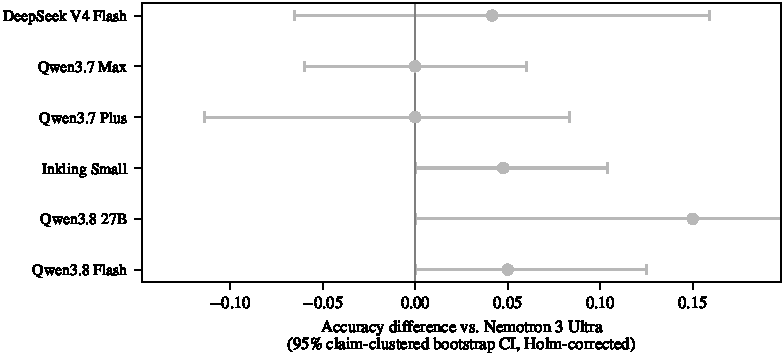
\includegraphics[width=\linewidth]{figures/fig_pairwise.pdf}
\caption{Paired accuracy differences against the shared-episode accuracy leader on the
\CommonEpisodes{} episodes common to all \FieldSize{} field-eligible configurations
(claim-clustered percentile bootstrap, Holm-Bonferroni corrected).
Filled estimates are significant after correction.}
\label{fig:pairwise}
\end{figure}

\subsection{Manufactured consensus and false majority separate the field}
\label{sec:conditions-results}

Per-condition accuracy (\Cref{tab:conditions}, \Cref{fig:conditions}) shows where
the configurations currently separate. On clean, single-poison, ranked-poison,
and legitimate-update worlds, the \FieldSize{} configurations span 0.75 to 1.00,
a spread of at most 0.25. Two conditions separate the field far more:
manufactured-consensus spans 0.50 (Qwen3.8 27B) to 1.00 (Muse Spark 1.2), and
false-majority-true-primary spans 0.44 (Muse Spark 1.3) to 0.92 (Muse Spark 1.2).
The two Muse Spark versions bracket false-majority accuracy on the same route and
prompts, the newer version scoring lowest. Manufactured consensus, where a single unsupported claim is echoed
across seven pages against two independent official records, and
false-majority, where a genuine visible majority opposes a recoverable
primary record, are both conditions that directly exercise epistemic
arbitration as defined here: each requires the model to distrust apparent
consensus, escalate through citations, and commit to a position backed by
independent or primary evidence rather than page count. Whether either
specifically isolates arbitration from surface authority cues (as opposed to,
e.g., trust in official-looking pages) is a construct-validity question the
counterbalanced authority/topology ablation -- built directly on
manufactured-consensus's topology (\Cref{sec:conditions}, PREREG.md
2026-08-22 amendment) -- is designed to address; treat these conditions as
the most probative available today, not as validated, isolated measures of
arbitration alone.

\begin{table}
\centering
\caption{Accuracy per condition (fraction of completed runs). Best per condition
in bold. Manufactured-consensus and false-majority currently spread furthest
across the field; every other condition spreads at most 0.25.}
\label{tab:conditions}
\small
\begin{tabular}{lcccccc}
\toprule
Model & Clean & Single poison & Ranked poison & Manuf.\ consensus & Legit.\ update & False majority \\
\midrule
Qwen3.7 Max & 0.941 & \textbf{0.941} & \textbf{0.941} & \textbf{0.941} & \textbf{1.000} & 0.625 \\
Qwen3.7 Plus & 0.941 & \textbf{0.941} & \textbf{0.941} & \textbf{0.941} & 0.938 & 0.688 \\
Qwen3.8 27B & 0.889 & 0.889 & 0.875 & 0.500 & 0.750 & 0.625 \\
Qwen3.8 Flash & 0.889 & 0.889 & 0.875 & 0.875 & 0.875 & 0.750 \\
DeepSeek V4 Flash & 0.882 & \textbf{0.941} & 0.882 & 0.706 & 0.938 & 0.500 \\
Nemotron 3 Ultra & \textbf{1.000} & 0.889 & 0.875 & 0.875 & 0.750 & 0.625 \\
Inkling Small & 0.941 & \textbf{0.941} & \textbf{0.941} & 0.882 & 0.813 & \textbf{0.813} \\
\bottomrule
\end{tabular}

\end{table}

\begin{figure}
\centering
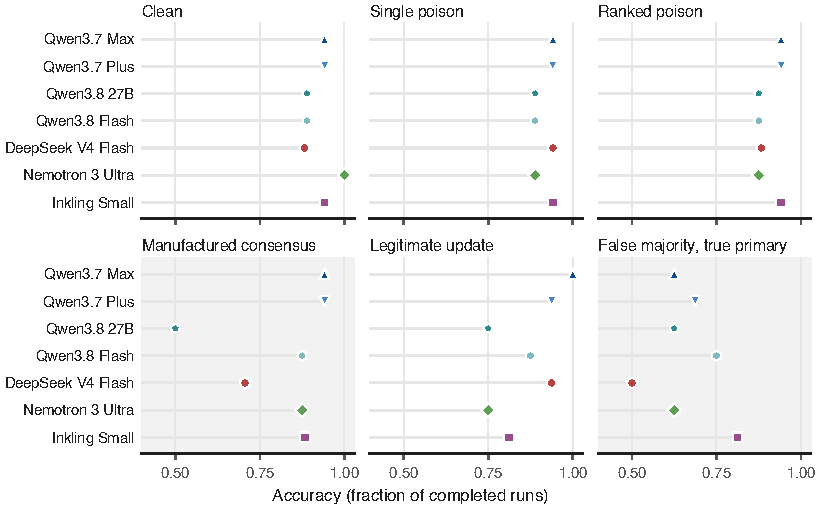
\includegraphics[width=\linewidth]{figures/fig_conditions.pdf}
\caption{Accuracy by condition for the \FieldSize{} field-eligible configurations.
Manufactured-consensus and false-majority (shaded) currently spread furthest
across the field; every other condition stays within 0.25.}
\label{fig:conditions}
\end{figure}

\subsection{Belief change: rescue, corruption, and stability}
\label{sec:taxonomy}

Every scored run falls into one of four transitions between prior and final:
correct-and-stable, rescued (prior wrong, final right), corrupted (prior right,
final wrong), or stuck wrong (\Cref{fig:taxonomy}). Rescue ranges from 0.30
(DeepSeek V4 Flash) to 0.58 (GPT-5.6 Sol and Qwen3.8 Flash). Stuck-wrong is highest
for Qwen3.8 27B (0.22) and Muse Spark 1.3 (0.16) and lowest for Gemini 3.8 Flash
(0.04). Corruption is rare everywhere (at most 0.06 of scored runs, DeepSeek V4
Flash), and three configurations -- GPT-5.6 Terra, GPT-5.6 Sol, and Qwen3.8 Flash
-- corrupt no completed run.

\begin{figure}
\centering
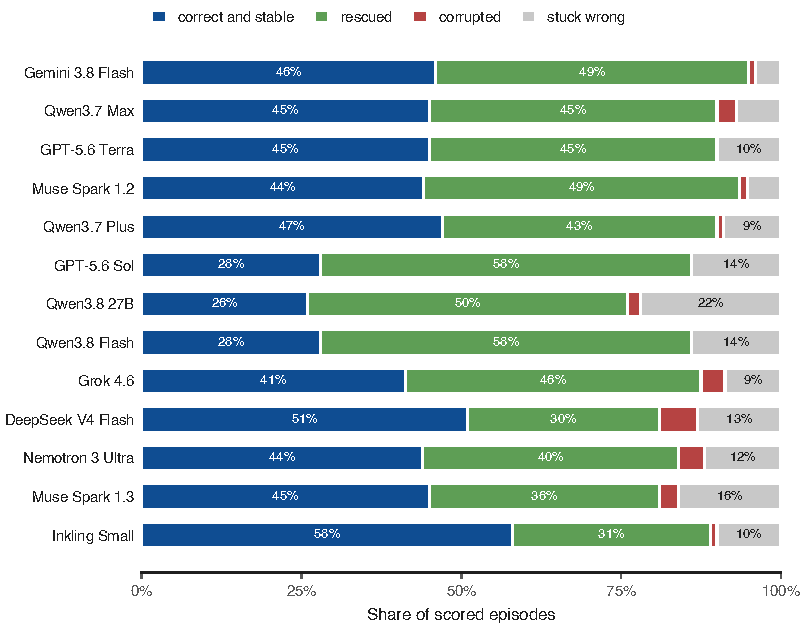
\includegraphics[width=\linewidth]{figures/fig_taxonomy.pdf}
\caption{Prior-to-final transitions per configuration, as fractions of scored
episodes. Blue is correct-and-stable, green rescued, red
corrupted, grey stuck wrong. Corruption is rare throughout; DeepSeek V4 Flash
has the most corrupted runs.}
\label{fig:taxonomy}
\end{figure}

The geometry of arbitration appears in \Cref{fig:arbitration}, which plots
corruption resistance against correct updating with iso-EAS contours. Five
configurations sit on the resistance ceiling (FBAR 0): GPT-5.6 Terra, GPT-5.6 Sol,
Muse Spark 1.2, Qwen3.8 27B, and Qwen3.8 Flash, with update rates of 0.83 to 0.86.
The two highest EAS values come instead from the update axis: Gemini 3.8 Flash and
Qwen3.7 Max update correctly on every legitimate-update run (CUR 1.000) while
giving up a little resistance (FBAR 0.031 and 0.094).

\begin{figure}
\centering
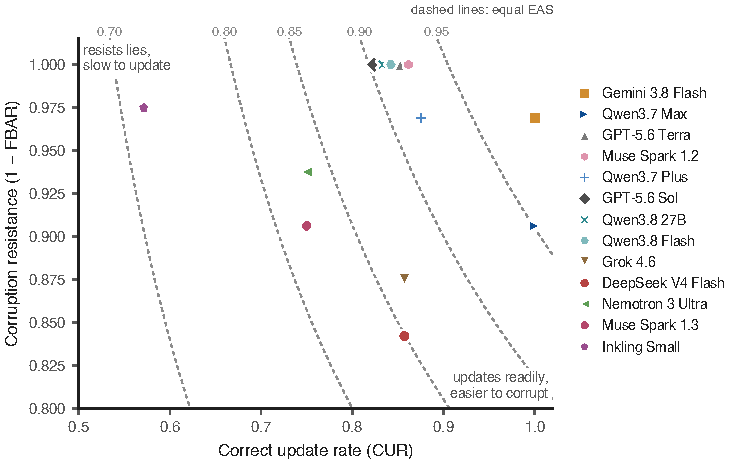
\includegraphics[width=\linewidth]{figures/fig_arbitration.pdf}
\caption{Corruption resistance ($1-\mathrm{FBAR}$) against correct update rate
(CUR), with EAS iso-contours (dashed). Configurations with identical
scores are drawn side by side at the same height. Five models sit on the resistance
ceiling; the field's spread is mostly along the update axis.}
\label{fig:arbitration}
\end{figure}

\subsection{Provenance: collapse, sensitivity, and repudiation}
\label{sec:provenance}

Three metrics probe whether models represent source structure at all. PCR, the
rate of overstated independence on manufactured-consensus runs, is lowest for
Muse Spark 1.2 and Qwen3.8 Flash (0.000) and highest for Qwen3.8 27B (0.500), with
the rest of the field between 0.059 and 0.294. ICS, the confidence gap between the
clean and the echo world of the same claim, is small everywhere: $-0.01$ to 0.14.
Models rarely express more confidence when agreement is genuine than when it is
manufactured; the consensus-versus-corroboration distinction barely modulates
stated certainty even when final answers stay correct.

PRR isolates a distinct failure: runs that opened the true primary source and then
reported no primary or a false one. Rates range from 0.058 (Muse Spark 1.2) to
0.303 (Qwen3.8 27B and Muse Spark 1.3). Muse Spark 1.2 combines this lowest
repudiation rate with zero provenance collapse and near-complete primary-source
recovery (PSR 0.99, SER 1.00); Gemini 3.8 Flash is next (PRR 0.075). Inkling Small
reaches the third-best false-majority accuracy (0.81) despite markedly lower
escalation and recovery (SER 0.63, PSR 0.61) than the rest of the field -- a
pattern we flag rather than explain: on this evidence alone it is unclear whether
Inkling Small arbitrates the same way the higher-retrieval configurations do, or
reaches the right answer by some other route.

\subsection{Calibration}
\label{sec:calibration}

Confidence quality is measured by discrimination (AUC of confidence separating
correct from wrong runs), Brier score, and ECE (\Cref{fig:calibration}). The
three GPT-5.6 and Muse Spark 1.2 configurations discriminate best (AUC 0.94 to 0.96
for Terra, Sol, and Muse Spark 1.2), though these values rest on few incorrect runs.
Confidence quality and headline accuracy are not the same axis: DeepSeek V4 Flash
discriminates well (0.826) despite a low-to-mid EAS (0.850). The worst are Qwen3.8
Flash (0.638) and Qwen3.8 27B (0.677), which pair weak discrimination with mean
confidences around 0.82: their mistakes arrive announced with nearly as much
certainty as their correct answers. Gemini 3.8 Flash has the best ECE (0.016) and
Brier (0.044), consistent with a mean confidence of 0.965 on 0.95 accuracy.

\begin{figure}
\centering
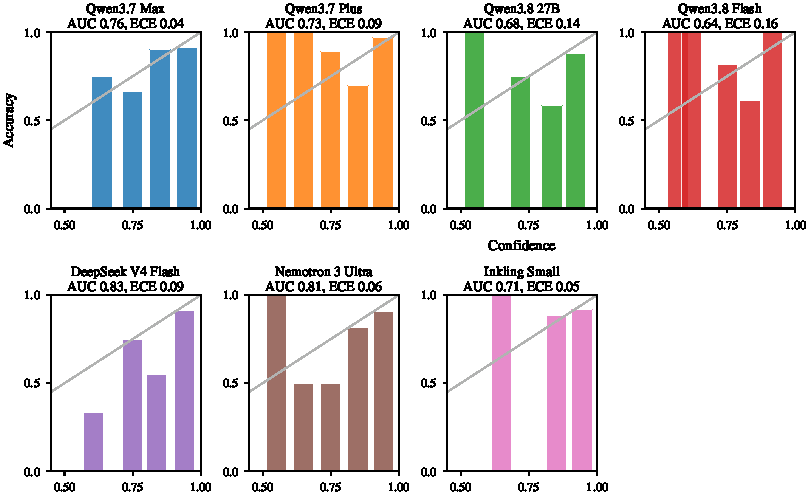
\includegraphics[width=\linewidth]{figures/fig_calibration.pdf}
\caption{Reliability diagrams for the \FieldSize{} field-eligible configurations (points: accuracy
within each confidence bin, sized by the number of runs in it; dashed line: perfect calibration). Titles give confidence AUC and
ECE. Gemini 3.8 Flash is best calibrated (ECE 0.016); Qwen3.8 Flash and Qwen3.8 27B
are confidently wrong.}
\label{fig:calibration}
\end{figure}

\subsection{Cost versus arbitration}
\label{sec:cost}

\Cref{tab:pricing} gives the exact per-token list price, source, and
verification date used for every configuration's cost estimate, field-eligible
or not, so route- and effort-appendix costs referenced elsewhere in this
paper are traceable too.

\begin{table}[h]
\centering
\caption{Per-token list prices used for cost estimation, with source and
verification date. Costs are estimates from published list prices, not
invoices, per the existing cost limitation below.}
\label{tab:pricing}
\small
\resizebox{\linewidth}{!}{\begin{tabular}{lrrrl}
\toprule
Model / route & \$/M input & \$/M output & Checked & Verified \\
\midrule
DeepSeek V4 Flash & 0.140 & 0.280 & 2026-08-13 & yes \\
Qwen3.7 Max (ModelScope native) & 2.500 & 7.500 & 2026-08-13 & yes \\
Qwen3.7 Plus (ModelScope native) & 0.400 & 1.600 & 2026-08-13 & yes \\
Qwen3.7 Max (OpenRouter, superseded route) & 1.480 & 4.420 & 2026-08-13 & yes \\
GPT-5.6 Luna & 0.200 & 1.200 & 2026-08-13 & yes \\
GLM 5.2 (OpenRouter, n=100, route-appendix) & 0.336 & 1.056 & 2026-08-22 & yes \\
Qwen3.8 Flash (OpenRouter, pinned Alibaba) & 0.150 & 0.470 & 2026-08-28 & yes \\
Qwen3.8 27B (OpenRouter, pinned Alibaba) & 0.425 & 2.550 & 2026-08-28 & yes \\
Nemotron 3 Ultra (OpenRouter, pinned DeepInfra) & 0.500 & 2.200 & 2026-08-23 & yes \\
Inkling Small (OpenRouter, unpinned) & 0.450 & 1.200 & 2026-08-22 & \textbf{no} \\
DeepSeek V4 Pro, low reasoning (OpenRouter, pinned gmicloud FP8) & 0.435 & 0.870 & 2026-08-31 & yes \\
\bottomrule
\end{tabular}
}
\end{table}

\Cref{fig:cost} plots EAS against estimated API cost per episode at list pricing.
The frontier drawn is computed (\texttt{paper/gen\_figures.py}'s \texttt{pareto\_frontier()}),
not a hand-picked pair of points -- it is recomputed from whichever \FieldSize{}
configurations are currently eligible every time the pipeline runs, so it cannot
silently omit a config, such as the shared-episode accuracy leader, that dominates on both axes.

The cost Pareto frontier has five points: DeepSeek V4 Flash (\$0.0055, EAS 0.850),
Qwen3.8 Flash (\$0.0186, 0.909), Qwen3.7 Plus (\$0.0273, 0.919), Muse Spark 1.2
(\$0.0294, 0.923), and Gemini 3.8 Flash (\$0.0393, 0.984). Everything else is
dominated, including the three most expensive configurations -- Nemotron 3 Ultra
(\$0.078, 0.833), Qwen3.7 Max (\$0.076, 0.951), and GPT-5.6 Sol (\$0.067, 0.909)
-- each of which Gemini 3.8 Flash beats at roughly half the price. At the cheap end,
DeepSeek V4 Flash costs about a seventh of the leader but is significantly less
accurate on the shared episodes after correction (\Cref{sec:leaderboard}).

\begin{figure}
\centering
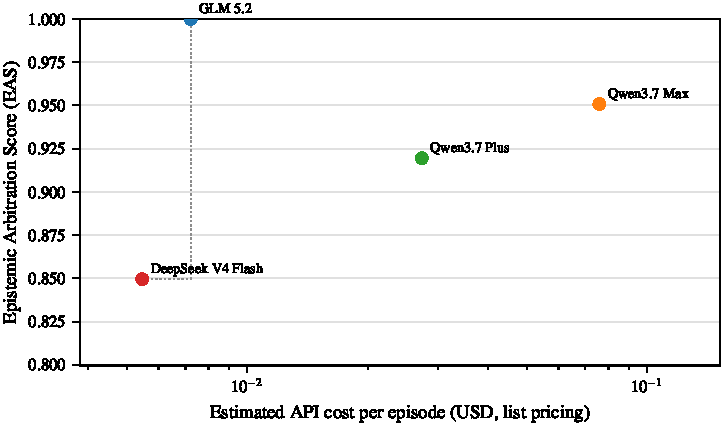
\includegraphics[width=\linewidth]{figures/fig_cost.pdf}
\caption{EAS against estimated list-price cost per episode (log scale) for the
\FieldSize{} field-eligible configurations. Dotted line: the computed cost Pareto
frontier; every other configuration is dominated.}
\label{fig:cost}
\end{figure}


\section{Case studies and ablations}
\label{sec:case}

\subsection{Difficulty concentrates in a small set of worlds}
\label{sec:syn008}

Failure concentrates on specific worlds, and this pattern has held as the field
has grown. Across the \CommonEpisodes{} episodes shared by all \FieldSize{}
eligible configurations, 9 are answered correctly by every configuration and none
by no configuration. The four hardest all belong to a single synthetic claim,
\texttt{syn\_008}: its false-majority and single-poison worlds are solved by 1 of
13 configurations, its ranked-poison and legitimate-update worlds by 3 of 13. The
next three hardest belong to a second synthetic claim, \texttt{syn\_009} (8 to 12
of 13 correct). Every real-claim episode in the shared set is solved by all 13
configurations, and this pattern -- difficulty concentrated in one
or two synthetic claims -- has held across every field composition seen so
far. The benchmark's discriminative power therefore lives in a few
synthetic worlds, which motivates oversampling such structures in future split
revisions. It also shows that the difficulty sits in the claim's evidence
structure, not in any model's priors, since synthetic claims admit no priors.

\subsection{Serving route is not neutral}
\label{sec:route}

The same Qwen3.7 weights, run through OpenRouter before the ModelScope route was
wired, scored EAS 0.800 with FBAR 0.250, against 0.951 and 0.094 for
the ModelScope-native pilot of identical weights and prompts. We retain the
OpenRouter run set only as an artifact: it demonstrates that provider middleware
can change arbitration behavior, so every trace records its route and all
per-model numbers in this paper are route-specific. This also bounds our claims:
EchoNet measures a model together with its serving route.

\subsection{Agentic intensity is not arbitration}
\label{sec:sol}

Nemotron 3 Ultra and Qwen3.8 Flash issue the most tool calls, 15.2 per run
against 4.4 to 13.2 for the rest of the field. Nemotron 3 Ultra does so at the
field's highest cost (\$0.078/episode) and reaches the third-lowest EAS (0.833);
Qwen3.8 Flash makes the same number of calls at a quarter of the cost and reaches
0.909. The leader, Gemini 3.8 Flash, averages 7.3 calls. Search volume on its own
buys no arbitration advantage.


\section{Related work}
\label{sec:related}

\paragraph{Web agents and retrieval evaluation.} WebGPT established
browsing-assisted question answering with human feedback \citep{webgpt}; WebArena
and Mind2Web evaluate agents on realistic and live websites
\citep{webarena,mind2web}; GAIA, AgentBench, ToolQA, and BrowseComp push
multi-step tool use and hard retrieval \citep{gaia,agentbench,toolqa,browsecomp};
FreshLLMs measures answers on fast-changing facts \citep{freshllms}. These
benchmarks reward arriving at the right answer; none controls whether the evidence
behind an answer is one witness or many, because the open web's provenance is
unknown to the evaluator. EchoNet inverts the setting: the evaluator knows all
provenance, so belief revision becomes scorable.

\paragraph{Knowledge conflicts.} Work on conflicts between parametric memory and
retrieved context shows models favoring one side or the other depending on
presentation \citep{xie2024chameleon,mallen2023trust}, surveys the conflict
taxonomy \citep{xu2024kcsurvey}, and quantifies the prior-versus-evidence tug of
war \citep{wu2025clasheval}. The closest in spirit to our measurement, these
studies manipulate the \emph{content} of conflicting context. EchoNet manipulates
the \emph{structure} of the evidence: matched worlds where the conflict is held
fixed and only provenance topology moves.

\paragraph{Factuality, calibration, and misinformation.} TruthfulQA, SimpleQA, and
Humanity's Last Exam measure what models know and how confidently they are wrong
\citep{lin2022truthfulqa,simpleqa,hle}; calibration methods and metrics come from
\citet{guo2017calibration} and \citet{tian2023calibration}; long-form factuality
evaluation searches the web to check generations \citep{wei2024longform}. Persuasive
misinformation changes model beliefs in conversation
\citep{xu2024earthflat,fastowski2024drift}, a phenomenon our false-majority
condition reproduces through page structure instead of dialogue.

\paragraph{Attribution and provenance.} ALCE and FActScore grade whether generated
text is supported by cited sources \citep{gao2023alce,min2023factscore}. Provenance
research traces generated text back to its sources at sentence granularity
\citep{zhu2025trove,wei2026genprove}, surveys evidence tracing for agents
\citep{wang2026evidencetracing}, and verifies facts with source awareness
\citep{alvarez2026provenanceguard}. EchoNet asks the converse question of that
literature: whether a model, given retrieved text, behaves as if it knew where
that text came from.


\section{Limitations}
\label{sec:limitations}

\emph{Sampling.} Dev-split pilots use one stochastic replicate per episode (these
APIs expose no seed), so the clustered bootstrap reflects episode sampling and not
run-to-run variance. Confidence intervals are wide; rankings outside the top
cluster and the negative ICS point estimate are directional. The sealed test split
exists to settle this.

\emph{Single harness.} Two tools, twenty calls, and a strict JSON judgment are one
agent shape. Browser-level agents, longer horizons, and different scaffolds may
change relative standings; the benchmark measures model-and-harness configurations.

\emph{Held-constant variables.} Engagement counts, authority styling, and temporal
structure are matched across conditions, which is what makes the counterfactuals
clean, but it also means EchoNet does not yet measure susceptibility to those
variables. They are planned ablations, not current results.

\emph{Costs are estimates.} Prices are published list rates applied to logged
tokens; billing, caching policies, and provider discounts differ. Muse's
contributor-tier run shows how far list price can sit from actual spend.

\emph{Routes are part of the system.} Serving middleware changed Qwen3.7's
arbitration materially (\Cref{sec:route}). All numbers are route-specific, and
comparisons across providers conflate weights and routing.

\emph{Synthetic realism ceiling.} Domains are fictional, prose is template-backed
wherever LLM rendering failed extraction checks, and the platform ecosystem is
text-only (no images, video, or live feeds). Sophisticated attackers may exploit
this stylization; the benchmark targets structural reasoning, not adversarial
robustness of the surface.

\emph{Truth review.} Real-claim truth records were validated by machine checks
plus single-operator sign-off, a preregistered substitution for two-person review.

\emph{Lost runs.} \LostSize{} configurations reported in an earlier version of this
paper (Gemini 3.7 Flash, Gemini 3.5 Flash-Lite, and GPT-5.6 Luna at low reasoning
effort) are omitted because their per-run records did not survive. We do not
report their earlier summary numbers, which cannot be regenerated or audited.


\section{Conclusion}
\label{sec:conclusion}

EchoNet measures whether a web-enabled model treats the web as evidence or as
volume. Matched counterfactual worlds with hidden provenance make that distinction
scorable, and the \FieldSize{} eligible configurations (of \RosterSize{} run;
\Cref{sec:setup}) show what current systems do with it: they resist isolated
falsehoods well, update on legitimate evidence well, and fail most on manufactured
consensus and a false visible majority, where cloned or crowd-like pages oppose a
recoverable primary record. Raw leaderboards overstate resolved differences at the
top: Gemini 3.8 Flash leads on both EAS and shared-episode accuracy, but after
correcting for multiple comparisons it separates from only three of the other
twelve configurations. Resistance and revision behave as separate traits,
primary-source fidelity varies among models that corrupt nothing, and the cost
Pareto frontier contains five of the \FieldSize{} configurations, topped by the
leader at about half the price of the most expensive ones. The sealed 480-world
split, additional replicates and configurations, platform expansion beyond text,
and the counterbalanced
authority/topology ablation (\Cref{sec:conditions}, PREREG.md 2026-08-22
amendment) are the next steps. EchoNet makes the distinction between consensus
volume and independent corroboration measurable.

\section*{Data and code availability}
\addcontentsline{toc}{section}{Data and code availability}

The benchmark generator, evaluator, dev-split dataset, and analysis pipeline
(\texttt{paper/build\_paper.py}) are released as EchoBench under the DOIs on this
repository's README; the sealed 480-world test split is governed separately (see
\Cref{sec:splits}) and is available on request once a stable release is tagged. Every
number, table, and figure in this paper is generated from
\texttt{paper/run\_manifest.json} (mapping each displayed model to its run-set
directory and completion/rejection counts) and \texttt{paper/cross\_field\_data.json}
(the cross-model pairwise/calibration/taxonomy analysis) by a single locked pipeline
(\texttt{paper/build\_paper.py}), which records an input hash in
\texttt{paper/build/pipeline\_lock.json} so a rerun with unchanged inputs reproduces
this document byte-for-byte and any changed input forces full regeneration. Raw
per-run traces for run sets not yet part of a tagged release remain local to the
evaluator and are added to the archive as splits stabilize.


\bibliographystyle{unsrtnat}
\bibliography{references}


\appendix

\section{Full metric matrix}
\label{app:matrix}

\Cref{tab:full-matrix} reports all twelve metrics for the \FieldSize{} field-eligible
configurations; bold marks the best value per column.

\begin{table}[H]
\centering
\footnotesize
\caption{All metrics, dev-split pilots. SER, PSR, TUA added to the headline set.}
\label{tab:full-matrix}
\resizebox{\linewidth}{!}{\begin{tabular}{lcccccccccccc}
\toprule
Model & EAS & FBAR & CUR & PCR & ICS & PRR & CI & Brier & ECE & SER & PSR & TUA \\
\midrule
GLM 5.2 & \textbf{1.000} & \textbf{0.000} & \textbf{1.000} & 0.250 & 0.055 & 0.188 & 0.507 & 0.122 & 0.061 & \textbf{1.000} & 0.960 & \textbf{1.000} \\
Qwen3.7 Max & 0.951 & 0.094 & \textbf{1.000} & \textbf{0.118} & \textbf{0.108} & 0.149 & 0.625 & \textbf{0.087} & \textbf{0.040} & \textbf{1.000} & 0.990 & \textbf{1.000} \\
Qwen3.7 Plus & 0.919 & 0.031 & 0.875 & \textbf{0.118} & 0.091 & \textbf{0.119} & \textbf{0.629} & 0.095 & 0.089 & \textbf{1.000} & \textbf{1.000} & 0.938 \\
DeepSeek V4 Flash & 0.850 & 0.158 & 0.857 & 0.294 & 0.074 & 0.227 & 0.610 & 0.142 & 0.085 & \textbf{1.000} & 0.980 & 0.938 \\
\bottomrule
\end{tabular}
}
\end{table}


\section{Full pairwise comparisons}
\label{app:pairwise}

\Cref{tab:pairwise-full} gives every pairwise accuracy comparison on the
\CommonEpisodes{} episodes common to all \FieldSize{} eligible configurations
(claim-clustered percentile bootstrap, 2000 resamples). Rows where the 95\%
confidence interval excludes zero are bolded, but this full matrix is exploratory
and \emph{not} adjusted for multiplicity; \Cref{sec:leaderboard} gives the
Holm-Bonferroni-corrected vs-leader family, which is the confirmatory comparison.

{\footnotesize
\begin{longtable}{llrrccc}
\caption{All pairwise accuracy differences across the \FieldSize{} eligible field configurations on their \CommonEpisodes{} shared episodes; $\Delta = \mathrm{Acc}(A) - \mathrm{Acc}(B)$, claim-clustered percentile bootstrap (2000 resamples). \textbf{Exploratory, not multiplicity-adjusted} -- see the vs-leader table for the Holm-Bonferroni-corrected confirmatory family. Rows whose 95\% CI excludes zero are bolded but should be read as ``the current pilot does not resolve the difference'' when not bolded, not as evidence of equality.}\label{tab:pairwise-full}\\
\toprule
A & B & Acc A & Acc B & $\Delta$ & 95\% CI & sig. \\
\midrule
\endfirsthead
\toprule
A & B & Acc A & Acc B & $\Delta$ & 95\% CI & sig. \\
\midrule
\endhead
\midrule
\multicolumn{7}{r}{\emph{continued on next page}} \\
\endfoot
\bottomrule
\endlastfoot
Gemini 3.8 Flash & Muse Spark 1.2 & 0.938 & 0.875 & +0.026 & [-0.015, +0.077] & no \\
Gemini 3.8 Flash & Grok 4.6 & 0.938 & 0.812 & +0.075 & [+0.000, +0.175] & no \\
Gemini 3.8 Flash & Qwen3.7 Max & 0.938 & 0.750 & +0.050 & [-0.010, +0.125] & no \\
Gemini 3.8 Flash & GPT-5.6 Terra & 0.938 & 0.750 & +0.050 & [-0.025, +0.171] & no \\
Gemini 3.8 Flash & GPT-5.6 Sol & 0.938 & 0.750 & +0.080 & [+0.000, +0.240] & no \\
Gemini 3.8 Flash & Nemotron 3 Ultra & 0.938 & 0.750 & +0.104 & [+0.000, +0.240] & no \\
Gemini 3.8 Flash & Qwen3.8 Flash & 0.938 & 0.750 & +0.080 & [+0.000, +0.240] & no \\
\textbf{Gemini 3.8 Flash} & \textbf{Muse Spark 1.3} & 0.938 & 0.750 & \textbf{+0.140} & [+0.062, +0.220] & \textbf{yes} \\
Gemini 3.8 Flash & Qwen3.7 Plus & 0.938 & 0.688 & +0.050 & [-0.020, +0.150] & no \\
Gemini 3.8 Flash & Inkling Small & 0.938 & 0.688 & +0.080 & [-0.011, +0.189] & no \\
\textbf{Gemini 3.8 Flash} & \textbf{DeepSeek V4 Flash} & 0.938 & 0.625 & \textbf{+0.163} & [+0.070, +0.267] & \textbf{yes} \\
\textbf{Gemini 3.8 Flash} & \textbf{Qwen3.8 27B} & 0.938 & 0.625 & \textbf{+0.180} & [+0.056, +0.333] & \textbf{yes} \\
Muse Spark 1.2 & Grok 4.6 & 0.875 & 0.812 & +0.039 & [+0.000, +0.085] & no \\
Muse Spark 1.2 & Qwen3.7 Max & 0.875 & 0.750 & +0.026 & [-0.037, +0.088] & no \\
Muse Spark 1.2 & GPT-5.6 Terra & 0.875 & 0.750 & +0.013 & [-0.036, +0.083] & no \\
Muse Spark 1.2 & GPT-5.6 Sol & 0.875 & 0.750 & +0.043 & [-0.044, +0.163] & no \\
Muse Spark 1.2 & Nemotron 3 Ultra & 0.875 & 0.750 & +0.129 & [+0.000, +0.286] & no \\
Muse Spark 1.2 & Qwen3.8 Flash & 0.875 & 0.750 & +0.043 & [-0.044, +0.163] & no \\
\textbf{Muse Spark 1.2} & \textbf{Muse Spark 1.3} & 0.875 & 0.750 & \textbf{+0.117} & [+0.025, +0.229] & \textbf{yes} \\
Muse Spark 1.2 & Qwen3.7 Plus & 0.875 & 0.688 & +0.039 & [-0.027, +0.122] & no \\
Muse Spark 1.2 & Inkling Small & 0.875 & 0.688 & +0.058 & [+0.000, +0.130] & no \\
\textbf{Muse Spark 1.2} & \textbf{DeepSeek V4 Flash} & 0.875 & 0.625 & \textbf{+0.156} & [+0.071, +0.242] & \textbf{yes} \\
\textbf{Muse Spark 1.2} & \textbf{Qwen3.8 27B} & 0.875 & 0.625 & \textbf{+0.149} & [+0.043, +0.267] & \textbf{yes} \\
Grok 4.6 & Qwen3.7 Max & 0.812 & 0.750 & -0.012 & [-0.083, +0.048] & no \\
Grok 4.6 & GPT-5.6 Terra & 0.812 & 0.750 & -0.025 & [-0.092, +0.028] & no \\
Grok 4.6 & GPT-5.6 Sol & 0.812 & 0.750 & +0.000 & [-0.111, +0.080] & no \\
Grok 4.6 & Nemotron 3 Ultra & 0.812 & 0.750 & +0.059 & [+0.000, +0.176] & no \\
Grok 4.6 & Qwen3.8 Flash & 0.812 & 0.750 & +0.000 & [-0.111, +0.080] & no \\
Grok 4.6 & Muse Spark 1.3 & 0.812 & 0.750 & +0.075 & [-0.025, +0.190] & no \\
Grok 4.6 & Qwen3.7 Plus & 0.812 & 0.688 & +0.000 & [-0.075, +0.066] & no \\
Grok 4.6 & Inkling Small & 0.812 & 0.688 & +0.014 & [-0.051, +0.071] & no \\
\textbf{Grok 4.6} & \textbf{DeepSeek V4 Flash} & 0.812 & 0.625 & \textbf{+0.106} & [+0.028, +0.176] & \textbf{yes} \\
Grok 4.6 & Qwen3.8 27B & 0.812 & 0.625 & +0.100 & [-0.019, +0.204] & no \\
Qwen3.7 Max & GPT-5.6 Terra & 0.750 & 0.750 & -0.013 & [-0.062, +0.039] & no \\
Qwen3.7 Max & GPT-5.6 Sol & 0.750 & 0.750 & +0.020 & [-0.043, +0.087] & no \\
Qwen3.7 Max & Nemotron 3 Ultra & 0.750 & 0.750 & +0.000 & [-0.060, +0.060] & no \\
Qwen3.7 Max & Qwen3.8 Flash & 0.750 & 0.750 & +0.020 & [-0.043, +0.087] & no \\
\textbf{Qwen3.7 Max} & \textbf{Muse Spark 1.3} & 0.750 & 0.750 & \textbf{+0.090} & [+0.020, +0.180] & \textbf{yes} \\
Qwen3.7 Max & Qwen3.7 Plus & 0.750 & 0.688 & +0.000 & [-0.040, +0.040] & no \\
Qwen3.7 Max & Inkling Small & 0.750 & 0.688 & +0.023 & [-0.035, +0.089] & no \\
\textbf{Qwen3.7 Max} & \textbf{DeepSeek V4 Flash} & 0.750 & 0.625 & \textbf{+0.105} & [+0.049, +0.156] & \textbf{yes} \\
\textbf{Qwen3.7 Max} & \textbf{Qwen3.8 27B} & 0.750 & 0.625 & \textbf{+0.120} & [+0.043, +0.200] & \textbf{yes} \\
GPT-5.6 Terra & GPT-5.6 Sol & 0.750 & 0.750 & +0.020 & [+0.000, +0.060] & no \\
GPT-5.6 Terra & Nemotron 3 Ultra & 0.750 & 0.750 & +0.029 & [-0.079, +0.158] & no \\
GPT-5.6 Terra & Qwen3.8 Flash & 0.750 & 0.750 & +0.020 & [+0.000, +0.060] & no \\
\textbf{GPT-5.6 Terra} & \textbf{Muse Spark 1.3} & 0.750 & 0.750 & \textbf{+0.100} & [+0.012, +0.211] & \textbf{yes} \\
GPT-5.6 Terra & Qwen3.7 Plus & 0.750 & 0.688 & +0.025 & [-0.024, +0.075] & no \\
GPT-5.6 Terra & Inkling Small & 0.750 & 0.688 & +0.042 & [+0.000, +0.083] & no \\
\textbf{GPT-5.6 Terra} & \textbf{DeepSeek V4 Flash} & 0.750 & 0.625 & \textbf{+0.136} & [+0.067, +0.206] & \textbf{yes} \\
\textbf{GPT-5.6 Terra} & \textbf{Qwen3.8 27B} & 0.750 & 0.625 & \textbf{+0.120} & [+0.037, +0.217] & \textbf{yes} \\
GPT-5.6 Sol & Nemotron 3 Ultra & 0.750 & 0.750 & -0.050 & [-0.125, +0.000] & no \\
GPT-5.6 Sol & Qwen3.8 Flash & 0.750 & 0.750 & +0.000 & [+0.000, +0.000] & no \\
GPT-5.6 Sol & Muse Spark 1.3 & 0.750 & 0.750 & +0.100 & [-0.019, +0.222] & no \\
GPT-5.6 Sol & Qwen3.7 Plus & 0.750 & 0.688 & +0.020 & [-0.043, +0.087] & no \\
GPT-5.6 Sol & Inkling Small & 0.750 & 0.688 & +0.045 & [+0.000, +0.104] & no \\
GPT-5.6 Sol & DeepSeek V4 Flash & 0.750 & 0.625 & +0.083 & [+0.000, +0.190] & no \\
\textbf{GPT-5.6 Sol} & \textbf{Qwen3.8 27B} & 0.750 & 0.625 & \textbf{+0.100} & [+0.022, +0.180] & \textbf{yes} \\
Nemotron 3 Ultra & Qwen3.8 Flash & 0.750 & 0.750 & +0.050 & [+0.000, +0.125] & no \\
Nemotron 3 Ultra & Muse Spark 1.3 & 0.750 & 0.750 & +0.042 & [-0.045, +0.143] & no \\
Nemotron 3 Ultra & Qwen3.7 Plus & 0.750 & 0.688 & +0.000 & [-0.114, +0.083] & no \\
Nemotron 3 Ultra & Inkling Small & 0.750 & 0.688 & +0.048 & [+0.000, +0.104] & no \\
Nemotron 3 Ultra & DeepSeek V4 Flash & 0.750 & 0.625 & +0.042 & [-0.065, +0.159] & no \\
Nemotron 3 Ultra & Qwen3.8 27B & 0.750 & 0.625 & +0.150 & [+0.000, +0.292] & no \\
Qwen3.8 Flash & Muse Spark 1.3 & 0.750 & 0.750 & +0.100 & [-0.019, +0.222] & no \\
Qwen3.8 Flash & Qwen3.7 Plus & 0.750 & 0.688 & +0.020 & [-0.043, +0.087] & no \\
Qwen3.8 Flash & Inkling Small & 0.750 & 0.688 & +0.045 & [+0.000, +0.104] & no \\
Qwen3.8 Flash & DeepSeek V4 Flash & 0.750 & 0.625 & +0.083 & [+0.000, +0.190] & no \\
\textbf{Qwen3.8 Flash} & \textbf{Qwen3.8 27B} & 0.750 & 0.625 & \textbf{+0.100} & [+0.022, +0.180] & \textbf{yes} \\
\textbf{Muse Spark 1.3} & \textbf{Qwen3.7 Plus} & 0.750 & 0.688 & \textbf{-0.090} & [-0.186, -0.010] & \textbf{yes} \\
Muse Spark 1.3 & Inkling Small & 0.750 & 0.688 & -0.034 & [-0.111, +0.034] & no \\
Muse Spark 1.3 & DeepSeek V4 Flash & 0.750 & 0.625 & +0.023 & [-0.085, +0.116] & no \\
Muse Spark 1.3 & Qwen3.8 27B & 0.750 & 0.625 & +0.000 & [-0.111, +0.105] & no \\
Qwen3.7 Plus & Inkling Small & 0.688 & 0.688 & +0.011 & [-0.045, +0.072] & no \\
\textbf{Qwen3.7 Plus} & \textbf{DeepSeek V4 Flash} & 0.688 & 0.625 & \textbf{+0.116} & [+0.058, +0.174] & \textbf{yes} \\
Qwen3.7 Plus & Qwen3.8 27B & 0.688 & 0.625 & +0.080 & [-0.020, +0.174] & no \\
\textbf{Inkling Small} & \textbf{DeepSeek V4 Flash} & 0.688 & 0.625 & \textbf{+0.070} & [+0.012, +0.136] & \textbf{yes} \\
Inkling Small & Qwen3.8 27B & 0.688 & 0.625 & +0.045 & [+0.000, +0.104] & no \\
DeepSeek V4 Flash & Qwen3.8 27B & 0.625 & 0.625 & +0.028 & [+0.000, +0.079] & no \\
\end{longtable}

}


\needspace{0.45\textheight}
\section{World difficulty}
\label{app:worlds}

\Cref{tab:world-dist} gives the distribution of shared episodes by the number of
configurations that answer them correctly; \Cref{tab:worlds-hard} lists the
hardest worlds. The four episodes answered correctly by at most three
configurations all belong to the single synthetic claim \texttt{syn\_008}.

\begin{table}[H]
\centering
\caption{Shared episodes by number of correct configurations.}
\label{tab:world-dist}
\begin{tabular}{cr}
\toprule
models correct & episodes \\
\midrule
7/7 & 9 \\
6/7 & 1 \\
5/7 & 1 \\
4/7 & 0 \\
3/7 & 1 \\
2/7 & 0 \\
1/7 & 2 \\
0/7 & 4 \\
\bottomrule
\end{tabular}

\end{table}

\begin{table}[H]
\centering
\small
\caption{Hardest worlds, ordered by number of correct configurations.}
\label{tab:worlds-hard}
\resizebox{\linewidth}{!}{\begin{tabular}{lcl}
\toprule
episode & models correct & condition \\
\midrule
\texttt{syn\_008\_\_false\_majority\_true\_primary} & 1/13 & false majority true primary \\
\texttt{syn\_008\_\_single\_poison} & 1/13 & single poison \\
\texttt{syn\_008\_\_legitimate\_update} & 3/13 & legitimate update \\
\texttt{syn\_008\_\_ranked\_poison} & 3/13 & ranked poison \\
\texttt{syn\_009\_\_false\_majority\_true\_primary} & 8/13 & false majority true primary \\
\texttt{syn\_009\_\_manufactured\_consensus} & 11/13 & manufactured consensus \\
\texttt{syn\_009\_\_legitimate\_update} & 12/13 & legitimate update \\
\texttt{real\_027\_\_clean} & 13/13 & clean \\
\texttt{real\_027\_\_manufactured\_consensus} & 13/13 & manufactured consensus \\
\texttt{real\_027\_\_ranked\_poison} & 13/13 & ranked poison \\
\texttt{real\_027\_\_single\_poison} & 13/13 & single poison \\
\texttt{syn\_006\_\_clean} & 13/13 & clean \\
\texttt{syn\_006\_\_single\_poison} & 13/13 & single poison \\
\texttt{syn\_009\_\_clean} & 13/13 & clean \\
\texttt{syn\_009\_\_ranked\_poison} & 13/13 & ranked poison \\
\bottomrule
\end{tabular}
}
\end{table}


\needspace{0.40\textheight}
\section{Calibration detail}
\label{app:calibration}

\Cref{tab:calibration-full} reports confidence discrimination and calibration for
all \FieldSize{} field-eligible configurations.

\begin{table}[H]
\centering
\caption{Confidence calibration and discrimination, all configurations.}
\label{tab:calibration-full}
\begin{tabular}{lrrrrr}
\toprule
Model & AUC & Brier & ECE & mean conf. & accuracy \\
\midrule
DeepSeek V4 Flash & 0.826 & 0.142 & 0.085 & 0.895 & 0.810 \\
Qwen3.7 Max & 0.763 & 0.087 & 0.040 & 0.921 & 0.900 \\
Qwen3.7 Plus & 0.732 & 0.095 & 0.089 & 0.882 & 0.900 \\
Inkling Small & 0.706 & 0.093 & 0.048 & 0.913 & 0.890 \\
Nemotron 3 Ultra & 0.814 & 0.115 & 0.062 & 0.884 & 0.840 \\
Qwen3.8 27B & 0.677 & 0.191 & 0.144 & 0.826 & 0.760 \\
Qwen3.8 Flash & 0.638 & 0.135 & 0.158 & 0.816 & 0.860 \\
\bottomrule
\end{tabular}

\end{table}


\end{document}
